\documentclass[a4j,12pt,dvipdfmx]{jsreport}

% 数式
\usepackage{amsmath,amsfonts}
\usepackage{bm}

% 画像
\usepackage[dvipdfmx,top=35truemm,bottom=30truemm,left=30truemm,right=30truemm]{geometry}
\usepackage[dvipdfmx]{graphicx}
% biblatex
\usepackage[style=numeric, sorting=none, maxbibnames=1000]{biblatex}
\addbibresource{graduation_thesis.bib}

% itembox
\usepackage{ascmac}
% breakitemboxのためのpackage
\usepackage{itembkbx}
% \usepackage{tcolorbox} 画像が見えなくなってしまう原因
% \usepackage{framed} 枠

% フォント
\usepackage[ipaex]{pxchfon}
\listfiles
\usepackage{float}
\usepackage{multicol}
\usepackage{multirow}
\usepackage{paralist}
\usepackage{caption}
% \captionsetup{format=plain, justification=centering}
\usepackage{setspace}
\usepackage{algorithm}
\usepackage{algpseudocode}
\usepackage[dvipdfmx,hidelinks]{hyperref}
\usepackage{pxjahyper}
\usepackage{fancyhdr}
\usepackage{ltablex}
\usepackage{capt-of}
\usepackage{tabularx}
\usepackage[export]{adjustbox}
\usepackage{booktabs}
\usepackage{enumitem} % itemizeの行間 これは下になければならない
\usepackage{threeparttable} % 表の脚注
\usepackage{titlesec}
\usepackage{makecell}
\usepackage{forest}
\usepackage{fancybox}
\usepackage{longtable}
\usepackage{xltabular}
% titlesec と \paragraph の相性問題を回避（run-in 見出しにする）
\titleformat{\paragraph}[runin]
  {\normalfont\normalsize\bfseries}
  {}{0pt}{} % ←ここには文字や \noindent 等を入れない
\titlespacing*{\paragraph}
  {0pt}{1.0ex}{0.8em}
\titleformat{\chapter}[hang]{\LARGE\bfseries}{\prechaptername\thechapter\postchaptername}{1em}{}

\setlength{\headheight}{16.5pt}
\captionsetup{format=hang}
\captionsetup[figure]{font=small}
\captionsetup[table]{font=small}
\begin{document}

% ▼▼▼ 仕掛け：main じゃないとき（単体のとき）だけヘッダー設定 ▼▼▼
\ifdefined\ismain\else
   \pagestyle{fancy}
   \lhead{\rightmark}
   \renewcommand{\chaptermark}[1]{\markboth{第\ \thechapter\ 章\ #1}{}}
   \setlength{\headheight}{16.5pt}
   \titleformat{\chapter}[hang]{\LARGE\bfseries}{\prechaptername\thechapter\postchaptername}{1em}{}
\fi
% ▲▲▲▲▲▲▲▲▲▲▲▲▲▲▲▲▲▲▲▲▲▲▲▲▲▲▲▲▲▲▲▲▲▲▲▲
\chapter{脚本に基づく漫画のネーム生成}
\label{chap:script2name}
本章では，構築したManga109NameDataset を用いて，
脚本に基づき漫画のネームを生成する手法について述べる．

本研究では，
ネームを，要素の幾何学的な配置を表すレイアウト情報（Layout）と
演出情報（Direction）が統合された，
物語と作品とを結ぶ中間表現として定義する．
Manga109NameDataset は，
この定義に基づき，
漫画画像に由来するネーム情報を
構造化データとして整理・構築したものである．

第~\ref{chap:script2layout}章で扱った脚本に基づくレイアウト生成では，
物語内容がコマや要素の配置にどのように反映されるかに着目していた．
これに対し本章では，Manga109NameDatasetを用いて
配置そのものに加え，
カメラワークやキャラクターの感情，
場面の雰囲気といった演出情報を含む
より包括的なネーム生成を対象とする．

すなわち本研究では，
脚本（Script）を入力とし，
演出情報（Direction）および
レイアウト情報（Layout）を生成することで，
脚本からネームへ至る生成過程を
計算機上で明示的に扱うことを目的とする．

本章の構成は以下の通りである．
まず~\ref{sec:script2name_formulation}節では，
脚本・演出情報・レイアウト情報からなる
ネーム生成タスクの問題設定を整理し，
定式化を行う．
次に~\ref{sec:script2name_method}節において，
脚本からネームを生成するための手法の概要を述べ，
演出情報およびレイアウト情報をどのように扱うかを説明する．
~\ref{sec:script2name_experiment}節では，
実験設定および評価方法について述べ，
最後に~\ref{sec:script2name_results}節で，
定量的および定性的な評価結果を示し，
脚本に基づくネーム生成の有効性について考察する．

\section{漫画のネーム生成における問題設定}
\label{sec:script2name_formulation}
本節では，
本研究における漫画のネーム生成タスクの問題設定を整理する．
特に，
脚本（Script）・演出情報（Direction）・レイアウト情報（Layout）からなる
三層構造の観点から，
本研究が対象とする生成問題を
脚本（Script）を入力とし，
演出情報（Direction）およびレイアウト情報（Layout）を生成する問題として定式化する． 図\ref{fig:script2name_formulation}にその概略図を示す．

\begin{figure}[htbp]
   \centering
   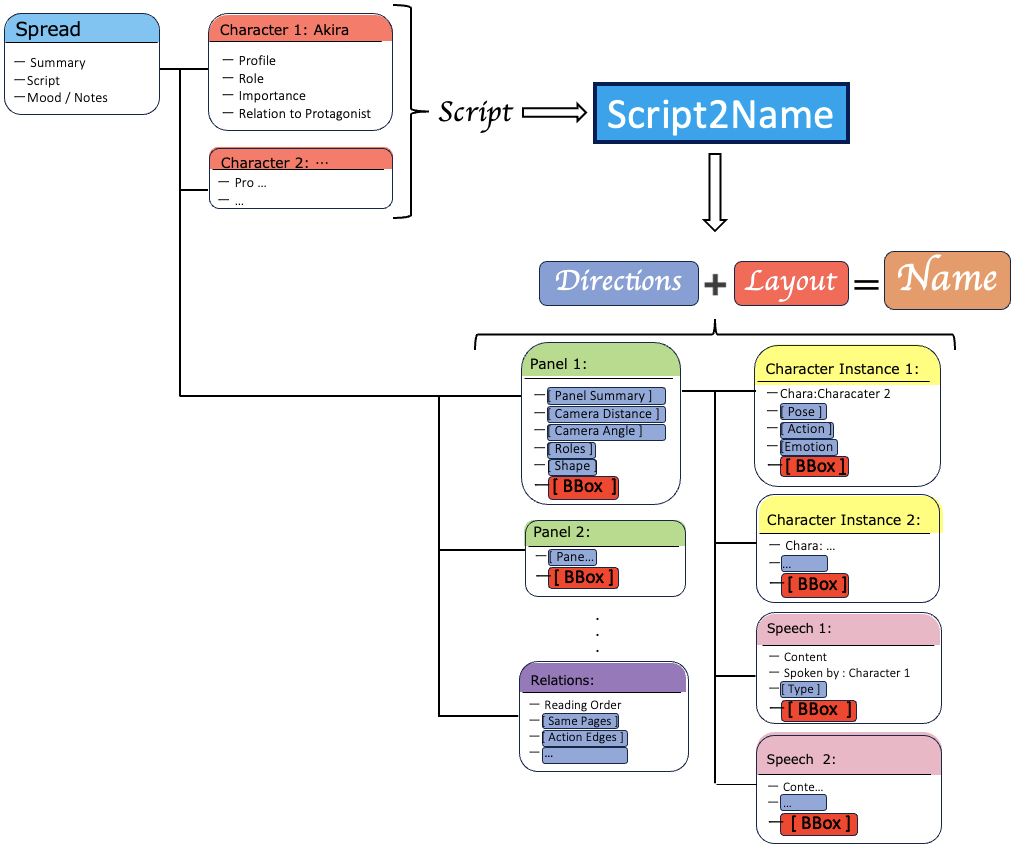
\includegraphics[width=\textwidth]{pict/06/script2name_formulation.png}
   \caption{脚本に基づく漫画ネーム生成タスクの概略図}
   \label{fig:script2name_formulation}
\end{figure}

\subsection{ネーム表現の定義}

本研究では，
第~\ref{chap:script2layout}章第~\ref{sec:problem_formulation}節で述べた
レイアウト表現を拡張し，
漫画のネームを，
$N \in \mathbb{N}$ 個の構成要素と，
場面全体に関わる演出情報からなる表現として定義する．
具体的には，
ネーム $n$ を
\[
   n = \left(
   \mathbf{d}^{\mathrm{global}},
   \{(c_1, \mathbf{d}_1, \mathbf{b}_1), \dots, (c_N, \mathbf{d}_N, \mathbf{b}_N)\}
   \right)
\]
と定義する．

ここで $c_i$ は $i$ 番目の要素のカテゴリを表し，
$\mathbf{d}_i$ はその要素に対応する局所的な演出情報，
$\mathbf{b}_i$ はページ平面上における位置と大きさを表す
バウンディングボックスである．
また，
$\mathbf{d}^{\mathrm{global}}$ は，
見開き全体や場面単位で共有される
グローバルな演出情報を表す．

カテゴリ $c_i$ は，
コマ，キャラクター，セリフといった
基本要素種別に基づくカテゴリ集合 $\mathcal{C}$ の要素であり，
$\mathcal{C}$ は
\[
   \mathcal{C}
   =
   \{\text{panel}\}
   \;\cup\;
   \{\text{character}_k\}
   \;\cup\;
   \{\text{speech}_k\}
\]
として定義される．

局所的な演出情報 $\mathbf{d}_i$ には，
キャラクターの姿勢や感情，
カメラ距離やアングルといった
要素単位で定義される演出属性が含まれる．
一方，
グローバルな演出情報 $\mathbf{d}^{\mathrm{global}}$ には，
主にノード間の関係において現れるエッジ情報
に紐づく演出情報が含まれる．
レイアウト情報 $\mathbf{b}_i$ は，
各要素のページ上での配置を表す
幾何学的情報である．

\subsection{ネーム生成タスクの定式化}

以上の定義のもと，
本研究におけるネーム生成タスクは，
脚本情報 $s$ が与えられたとき，
対応するネーム $n$ を生成する
条件付き生成問題として定式化される．
すなわち，
\[
   f : s
   \;\mapsto\;
   \left(
   \mathbf{d}^{\mathrm{global}},
   \{(c_i, \mathbf{d}_i, \mathbf{b}_i)\}_{i=1}^{N}
   \right)
\]
を学習することが目的である．

第~\ref{chap:script2layout}章で扱った
脚本に基づくレイアウト生成では，
$\mathbf{b}_i$ のみを生成対象としていたのに対し，
本章では，
局所的およびグローバルな演出情報 $\mathbf{d}_i$，
$\mathbf{d}^{\mathrm{global}}$ と
レイアウト情報 $\mathbf{b}_i$ を
統合的に生成する点が異なる．
これにより，
脚本に含まれる物語的文脈が，
配置設計だけでなく，
場面全体および要素単位の演出上の意思決定に
どのように反映されるかを
明示的に扱うことが可能となる．

\section{脚本に基づく漫画のネーム生成手法}
\label{sec:script2name_method}

本節では，
前節で定式化した脚本に基づく漫画のネーム生成タスクに対し，
本研究で用いた生成手法の概要を述べる．
本研究では，
脚本（Script）を入力とし，
演出情報（Direction）および
レイアウト情報（Layout）を
自然言語系列として出力する
LLM に基づくネーム生成手法を構築した．

基本的な枠組みは，
第~\ref{chap:script2layout}章で述べた
脚本に基づくレイアウト生成手法と同様に，
LLMを
教師あり学習によりファインチューニングするものである．
すなわち，
脚本表現をトークン列として入力し，
対応するネーム表現を
自己回帰的に出力するモデルを構築した．

入力となる脚本 $S$ は，
柱，ト書き，およびセリフを含む
見開き単位の脚本全文に加え，
脚本に登場するキャラクターの
プロフィールや役割といった
キャラクター設定を含む
自然言語列として与えられる．
これにより，
モデルは物語の進行だけでなく，
キャラクターの性格や立場といった
文脈情報を条件として利用できる．

ネーム生成においては，
LLM による生成および学習を可能にするため，
入力および出力を
あらかじめ定めた JSON 形式に基づいて線形化し，
トークン列として表現する．

具体的には，
ネームの構造を表す JSON テンプレートを事前に定義し，
コマ，キャラクターインスタンス，セリフといった
各要素に対応するフィールドを所定の位置に配置する．
モデルは，
このテンプレート構造を条件として，
演出情報（Direction）および
レイアウト情報（Layout）に対応するフィールドを
逐次生成する．

このとき，
ネームを構成する要素集合
$\{(c_i, \mathbf{d}_i, \mathbf{b}_i)\}_{i=1}^{N}$ は，
JSON 構造に沿って列挙され，
系列
\[
   \mathcal{N} = (\nu_1, \nu_2, \dots, \nu_T)
\]
として表現される．
各トークン $\nu_t$ は，
単一の要素に対応する
\[
   \nu_t = (c_{\pi(t)}, \mathbf{d}_{\pi(t)}, \mathbf{b}_{\pi(t)})
\]
として定義され，
$\pi(t)$ は
ネームを構成する全要素を
一度ずつ列挙する写像である．

演出情報 $\mathbf{d}_i$ は，
キャラクターの姿勢や感情，
カメラ距離やアングル，
コマの役割といった
要素単位で定義される演出属性の集合であり，
自然言語または離散的な記号列として表現される．
また，
見開き全体や場面単位で共有される
グローバルな演出情報
$\mathbf{d}^{\mathrm{global}}$ についても，
同様に JSON テンプレート内の所定の位置に配置し，
系列生成の一部として扱う．

レイアウト情報 $\mathbf{b}_i$ は，
各要素のページ平面上での位置と大きさを表す
バウンディングボックス
$\mathbf{b}_i = (x_i, y_i, w_i, h_i)$ として定義され，
脚本に基づくレイアウト生成と同様に，
あらかじめ定義した格子上に量子化された
離散トークンとして出力される．

学習時には，漫画のレイアウト生成手法と同様に，
脚本列 $S$ と，
それに対応する正解ネーム列 $\mathcal{N}$ からなる
教師データを用い，
LLM による条件付き確率
\[
   p_{\theta}(\mathcal{N} \mid S)
   =
   \prod_{t=1}^{T}
   p_{\theta}(\nu_t \mid \nu_{<t}, S)
\]
を最大化するように，
モデルパラメータ $\theta$ を最適化する．
損失関数としては，
次トークン予測に基づく
クロスエントロピー損失を用いる．

以上のように，
本研究では，
キャラクター設定を含む脚本を入力とし，
演出情報およびレイアウト情報を
構造化された形式で生成することで，
物語内容と演出設計とを統合した
ネーム生成を，
LLM による条件付き系列生成として実現する．

\section{漫画のネーム生成における実験設定}
\label{sec:script2name_experiment}
本節では，
脚本に基づくネーム生成手法の有効性を検証するために行った
実験設定について述べる．
具体的には，
実験に用いた Manga109NameDataset に含まれる
脚本（Script），演出情報（Direction），レイアウト情報（Layout）の構成を整理した上で，
これらの情報をどのように入力・出力として扱うかを定義する生成設定を説明する．
さらに，
データセット分割，
比較に用いたモデル，
学習および実装条件，
ならびに評価方法について順に述べる．

\subsection{データセットと入力・出力の整理}

本研究では，
脚本からネームを生成する過程を扱うにあたり，
まずデータセット内に含まれる情報を，
脚本（Script），演出情報（Direction），
およびレイアウト情報（Layout）という
三層構造の観点から整理する．
これは，
どの情報を入力として与え，
どの情報を生成対象とするかを
明確に定義するための前提となる．

Manga109NameDataset に含まれる主要なノードおよび属性を，
この三層構造に基づいて分類した結果を
表~\ref{tab:sdl_mapping} に示す．
Script 層には，
見開き全体の脚本本文に加え，
登場キャラクターのプロフィールや役割といった
グローバルな物語文脈に関わる情報が含まれる．
Direction 層には，
各コマやキャラクターインスタンスに対応する
演出上の意思決定を表す属性，
ならびにコマ間・キャラクター間の関係を表す
構造的情報が含まれる．
Layout 層は，
これらの要素がページ平面上で
どの位置・大きさに配置されるかを表す
幾何学的情報から構成される．

\begin{xltabular}{\textwidth}{ll >{\raggedright\arraybackslash}p{4.0cm} >{\small}X}

   % --- 最初のページのヘッダー ---
   \caption{Manga109NameDataset におけるScript/Direction/Layout構成の整理} \label{tab:sdl_mapping} \\
   \toprule
   \textbf{層} & \textbf{ノード} & \textbf{フィールド} & \textbf{内容} \\
   \midrule
   \endfirsthead

   % --- 2ページ目以降のヘッダー ---
   \caption[]{Manga109NameDataset における主要フィールドの構成（続き）} \\
   \toprule
   \textbf{層} & \textbf{ノード} & \textbf{フィールド} & \textbf{内容} \\
   \midrule
   \endhead

   % --- フッター（次ページへ続く...） ---
   \bottomrule
   \multicolumn{4}{r}{\small\textit{次ページへ続く...}} \\
   \endfoot

   % --- 最終フッター ---
   \bottomrule
   \endlastfoot

   % --- データ本体 ---
   \multirow{7}{*}{Script}
   & Spread
   & summary, script, \newline mood, notes
   & 見開き全体の要約・脚本（柱/ト書き/セリフ）・雰囲気・補足 \\
   \addlinespace
   & Character
   & name, profile, role, \newline importance, alignment, \newline \texttt{relation\_to\_protagonist}
   & キャラクター設定（プロフィール、役割、重要度、主人公との関係など） \\
   \addlinespace
   & Speech
   & text, \texttt{speaker\_id}
   & セリフ本文と話者識別ID \\
   \addlinespace
   & Structure
   & \texttt{panel\_ids}
   & 脚本中で言及されるパネルID列 \\
   \midrule
   \multirow{15}{*}{Direction}
   & Panel
   & summary
   & 各コマの内容要約（視覚的説明） \\
   & Panel
   & \texttt{roles} (categorical)
   & コマの役割（dialogue, reaction等） \\
   & Panel
   & \texttt{shape\_type}
   & コマ形状（standard, inset等） \\
   & Panel
   & \texttt{cinematic.distance}, \newline \texttt{cinematic.angle}
   & カメラ距離・アングル \\
   \addlinespace
   & Char. Inst.
   & pose, action, emotion
   & 姿勢・動作・感情（自由記述テキスト） \\
   & Char. Inst.
   & \texttt{pose}, \texttt{action}, \newline \texttt{emotion}, \texttt{face\_body} \newline (all categorical)
   & 姿勢・動作・感情・描写範囲（離散カテゴリ） \\
   \addlinespace
   & Speech
   & \texttt{type} (categorical)
   & セリフ種別（dialogue, monologue等） \\
   \addlinespace
   & Edges
   & \texttt{panel\_edges}
   & コマ間関係（順序や同一ページ判定） \\
   & Edges
   & \texttt{action\_edges}
   & キャラクター間相互作用（source/target/action） \\
   & Edges
   & \texttt{anchored\_to}
   & セリフのアンカー（Speech $\to$ Character） \\
   & Edges
   & \texttt{contains} (pred.)
   & Panel $\to$ Speech/Character の包含関係（予測） \\
   \midrule
   \multirow{5}{*}{Layout}
   & Panel
   & \texttt{bbox}
   & バウンディングボックス $\mathbf{b}_i=(x,y,w,h)$ \\
   & Char. Inst.
   & \texttt{bbox}
   & 同上（キャラクター位置） \\
   & Speech
   & \texttt{bbox}
   & 同上（セリフ位置） \\

\end{xltabular}

このように Script / Direction / Layout を整理した上で，
本研究では，
脚本からネームを生成する際の
情報生成の関係性を検証するため，
入力と出力の組み合わせが異なる
複数の生成設定を比較した．
表~\ref{tab:script2name_settings} に，
本研究で検討した 4 つの生成設定を示す．
これらの設定は，
脚本のみを入力としてレイアウトを生成する設定から，
演出情報とレイアウトを同時に生成する設定，
さらに演出情報を中間表現として経由する
段階的生成設定まで，
ネーム生成における生成粒度と生成順序が
異なる点で区別される．
特に，
Script2Name (Joint) は
演出情報とレイアウト情報を統合的に生成する設定であり，
Script2Direction2Layout は
演出情報を明示的な中間表現として導入することで，
段階的生成の有効性を検証するための設定である．

\begin{table}[htbp]
   \centering
   \caption{脚本に基づくネーム生成の比較設定．GNNはGraphical Neural Networkを表す．}
   \label{tab:script2name_settings}

   % 1. 文字サイズを小さくする (small より小さい footnotesize も検討)
   \small

   % 2. 列間隔を詰める (標準は6pt。ここでは3ptに半減)
   \setlength{\tabcolsep}{3pt}

   \begin{tabular}{lccc}
      \toprule
      \textbf{設定名} & \textbf{入力}                    & \textbf{出力} & \textbf{モデル構成} \\
      \midrule
      Script2Layout
                   & Script
                   & Layout
                   & LLM                                                           \\
      \addlinespace
      Script2Name (Joint)
                   & Script
                   & Direction + Layout
                   & LLM                                                           \\
      \addlinespace
      (Script+Direction)2Layout
                   & Script + Direction
                   & Layout
                   & LLM                                                           \\
      \addlinespace
      Script2Direction2Layout
                   & Script
                   & Direction $\rightarrow$ Layout
                   & LLM + GNN                                                     \\
      \bottomrule
   \end{tabular}
\end{table}



本研究では，これらの設定に基づき，
脚本からネーム生成へ至る過程を
異なる情報分解および生成順序の観点から比較する．
これらの生成設定は，
実際の漫画制作において，
演出を先に検討する場合や，
配置設計と演出を同時に検討する場合など，
制作工程や作家の作業スタイルに応じて
ネームの設計手順が異なる状況を抽象化したものである．
このような複数の生成設定を通じて，
脚本からネームを構築する際に，
演出情報をどの段階でどのように扱うことが有効であるかを
体系的に検証する．

\subsection{データセット分割}
学習に用いたManga109NameDatasetは，作品単位で分割し，
同一作品が訓練用・検証用・テスト用データにまたがらないようにした．
分割比は 8:1:1
訓練用データ 7{,}937 見開き，
検証用データ 1{,}113 見開き，
テスト用データ 991 見開きを用いた．

訓練用データは各生成設定におけるモデルの学習に，
検証用データは学習の早期終了およびモデル選択に用い，
最終的な性能評価はテスト用データ上で行った．
なお，
データセット分割および前処理の方針は，
第~\ref{chap:script2layout}章のレイアウト生成実験と同一である．

\subsection{比較手法}
脚本に基づくネーム生成手法の有効性の検証においても
第~\ref{chap:script2layout}章のレイアウト生成実験と同様，
既存のレイアウト生成手法との比較を行った．
比較に用いた手法も同じく，
LayoutDM~\cite{inoue2023layoutdm}，
LayoutFormer++~\cite{jiang_layoutformer_2023}，
LayoutPrompter~\cite{lin_layoutprompter_2023}
の 3 手法である．
これらの既存手法は，
ネーム生成における比較においても，要素カテゴリ情報を入力条件として与える Gen-T条件での生成に用い，脚本を条件とする生成条件にあわせてレイアウト生成性能の比較に用いた．

ほか学習の設定や推論の設定は，グリッド条件を見開き単位に対応させることを除いて第~\ref{chap:script2layout}章のレイアウト生成実験と同様である．

\subsection{ネーム生成における学習設定および実装詳細}
本節では，
表~\ref{tab:script2name_settings} に示した各生成設定において用いた
モデル構成と学習条件，ならびに実装上の設定について述べる．
LLM による生成設定である Script2Layout / Script2Name (Joint) / (Script+Direction)2Layout では，
教師ありファインチューニングを行った．
一方，段階的生成設定 Script2Direction2Layout では，
演出情報の生成に LLM をファインチューニングし，
レイアウト生成にはグラフニューラルネットワーク（GNN）を用いた．

\paragraph{LLM の選定}
本実験では，LLM として \texttt{gpt-oss-20b}，\texttt{Qwen3-14B}，\texttt{Llama-3.1-8B} を選定した．
これらはいずれも公開モデルの中で比較的新しく，
汎用的な言語能力において高い評価を得ていることから採用した．
複数の基盤モデルを用いることで，
モデル規模や事前学習の差異がネーム生成性能に与える影響を検証した．
学習は，各見開きの脚本（および条件に応じて演出情報）を入力とし，
JSON 形式に線形化した出力列を教師信号として，
次トークン予測に基づくクロスエントロピー損失を最小化することで行った．
学習手順は，第~\ref{chap:script2layout}章のレイアウト生成と同様である．

\paragraph{GNN によるレイアウト生成（Script2Direction2Layout）}
段階的生成設定 Script2Direction2Layout では，
まず LLM により脚本から演出情報（Direction）を生成し，
得られた Direction を条件として
GNN によりレイアウト（BBox）を推定した．
GNN は，見開きを表す異種グラフを入力とする HeteroConv に基づくモデルとして実装し，
ノード種別は Spread / Panel / Character / Character Instance / Speech とした．
エッジには，キャラクターインスタンス間の相互作用（action edges），
Panel と Character Instance の包含関係，
Speech の読順関係など，
Manga109NameDataset に含まれる主要な関係情報を用いた．
各ノードには，対応するテキスト特徴および演出属性を付与し，
メッセージパッシングによって特徴を更新した後，
Panel，CharacterInstance，Speech の各ノードに対して
混合密度ネットワーク（MDN）を用いてバウンディングボックスを推定した．

\paragraph{レイアウト表現の量子化と座標系}
レイアウト情報は，
各要素のバウンディングボックス
$\mathbf{b}_i = (x_i, y_i, w_i, h_i)$
として表現される．
LLM および GNN による生成を可能にするため，
これらの連続値座標は，
あらかじめ定義した格子上に量子化された
離散トークンとして扱った．

第~\ref{chap:script2layout}章のレイアウト生成では
ページ単位の生成を対象としていたため，
座標系を $32 \times 32$ の格子として定義していたのに対し，
本章では見開き単位のネーム生成を扱うことから，
横方向の表現範囲を拡張し，
$64 \times 32$ の格子を用いた．
これにより，
見開き全体を一貫した座標系で表現しつつ，
既存のレイアウト生成手法との整合性を保った．

\subsection{評価方法}
本研究では，
脚本に基づくネーム生成手法の有効性を検証するため，
主としてレイアウト生成結果に対する定量評価を行った．
レイアウトに関する評価指標および評価手順は，
第~\ref{chap:script2layout}章で用いたものと同一であり，
mIoU，FID，LTSim，LTSim-MMD を用いた．
これらの指標により，
要素の位置や大きさといった
幾何的配置の再現性を，
正解レイアウトとの比較に基づいて評価した．
そのため，
本章では各評価指標の詳細な定義については省略する．

一方で，
演出情報（Direction）については，
直接的な定量評価は行っていない．
これは，
Direction がカメラワーク，感情表現，場面の雰囲気といった
高次の意味的・主観的要素を含むため，
単一の数値指標として妥当な正解度を定義することが
現時点では困難であるためである．

そこで本研究では，
演出情報の生成結果について，
二つの観点から評価を行った．
第一に，
生成された Direction を
ノードおよび関係からなるグラフ構造として可視化し，
対応する正解データと比較することで，
キャラクター配置関係や
演出上の役割分担が
脚本内容と整合しているかを
定性的に分析した．

第二に，
段階的生成設定 Script2Direction2Layout においては，
Direction を入力としてレイアウトを生成する
グラフニューラルネットワーク（GNN）を評価器として用い，
生成された Direction の妥当性を
間接的に評価した．
具体的には，
同一の GNN に対して，
正解 Direction および
LLM により生成された Direction をそれぞれ入力し，
得られたレイアウト結果を
正解レイアウトと比較することで，
Direction がレイアウト生成に提供する
構造的情報の再現性を評価した．
この評価は，
Direction の意味内容そのものを直接測定するものではないが，
下流タスクであるレイアウト生成に対して
どの程度有効な情報を保持しているかを
定量的に比較するための指標として位置づけられる．

以上の評価方法により，
本研究では，
ネーム生成における
レイアウトの幾何的再現性と，
演出情報の構造的妥当性の双方について，
定量的および定性的な観点から分析を行った．
演出情報に対する
より直接的な定量評価指標の設計については，
今後の課題とする．

\section{漫画のネーム生成における結果と考察}\label{sec:script2name_results}
本節では，
前節で述べた各生成設定に基づく実験結果をもとに，
脚本に基づくネーム生成における
レイアウト生成性能および
生成設定の違いが与える影響について考察する．
特に，
既存のレイアウト生成手法との比較，
LLM に基づく各生成設定の傾向，
演出情報の統合方法の違い，
および段階的生成における課題の観点から結果に付いて考察する．

\subsection{漫画のネーム生成における定量的結果と考察}
表~\ref{tab:script2name_results_layout} に，ネーム生成におけるレイアウト生成性能の定量的結果を示す．

\begin{table*}[t]
   \captionsetup{font=small}
   \caption{
      脚本に基づくネーム生成におけるレイアウト生成の定量評価結果（見開き単位）．
   }
   \vspace{-0.6em}
   \centering
   \label{tab:script2name_results_layout}
   \setlength{\tabcolsep}{6pt}
   \begin{adjustbox}{max width=\textwidth}
      \begin{tabular}{l c c c c}
         \toprule
                                                           &
         \multicolumn{2}{c}{\textbf{Spread-level metrics}} &
         \multicolumn{2}{c}{\textbf{Distribution-level metrics}}                                                                                                              \\
         \cmidrule(lr){2-3} \cmidrule(lr){4-5}
         \textbf{Model}                                    &
         mIoU $\uparrow$                                   & LTSim $\uparrow$                                    &
         FID $\downarrow$                                  & \makecell{LTSim-MMD ($\times 10^{-2}$)$\downarrow$}                                                              \\
         \midrule

         \multicolumn{5}{l}{\itshape Existing layout generation methods (Category-conditioned)}                                                                               \\

         LayoutDM
                                                           & 0.0989                                              & 0.7064             & 54.095            & \underline{0.645} \\
         LayoutFormer++
                                                           & 0.0325                                              & 0.5632             & 56.520            & 5.258             \\
         LayoutPrompter
                                                           & 0.0964                                              & 0.6739             & 64.941            & 1.912             \\
         \midrule

         \multicolumn{5}{l}{\itshape Script2Direction2Layout (Fine-tuned LLM $\rightarrow$ GNN)}                                                                              \\

         GPT-OSS-20B
                                                           & 0.0851                                              & 0.7123             & 78.45             & 2.19              \\
         Llama-3.1-8B
                                                           & 0.0772                                              & 0.7055             & 105.10            & 3.75              \\
         Qwen3-14B
                                                           & 0.0822                                              & 0.7106             & 74.97             & 2.35              \\
         \midrule

         \multicolumn{5}{l}{\itshape (Script + Direction) $\rightarrow$ Layout (Fine-tuned LLM)}                                                                              \\

         GPT-OSS-20B
                                                           & 0.1086                                              & \underline{0.7484} & 14.52             & 0.71              \\
         Llama-3.1-8B
                                                           & 0.0162                                              & 0.4212             & 165.30            & 64.17             \\
         Qwen3-14B
                                                           & 0.1178                                              & \textbf{0.7711}    & \textbf{9.21}     & \textbf{0.50}     \\
         \midrule

         \multicolumn{5}{l}{\itshape Script $\rightarrow$ (Direction + Layout) (Fine-tuned LLM, Joint)}                                                                       \\

         GPT-OSS-20B
                                                           & \underline{0.1201}                                  & 0.7360             & 19.76             & 1.04              \\
         Llama-3.1-8B
                                                           & 0.0140                                              & 0.4154             & 168.78            & 64.68             \\
         Qwen3-14B
                                                           & 0.1254                                              & 0.7434             & 19.72             & 0.90              \\
         \midrule

         \multicolumn{5}{l}{\itshape Script2Layout (Fine-tuned LLM)}                                                                                                          \\

         GPT-OSS-20B
                                                           & 0.1177                                              & 0.7333             & 18.88             & 1.24              \\
         Llama-3.1-8B
                                                           & 0.0142                                              & 0.4165             & 166.84            & 64.06             \\
         Qwen3-14B
                                                           & \textbf{0.1269}                                     & 0.7421             & \underline{18.72} & 0.87              \\
         \bottomrule
      \end{tabular}
   \end{adjustbox}
\end{table*}


\paragraph{既存レイアウト生成手法との比較}

\paragraph{LLM に基づくネーム生成手法の全体的傾向}
...

\paragraph{演出情報の統合方法による違い}
...

\paragraph{段階的生成（Script2Direction2Layout）の限界}

% ▼▼▼ 仕掛け：main じゃないとき（単体のとき）だけ参考文献を表示 ▼▼▼
\ifdefined\ismain\else
   \printbibliography[title=参考文献]
\fi
% ▲▲▲▲▲▲▲▲▲▲▲▲▲▲▲▲▲▲▲▲▲▲▲▲▲▲▲▲▲▲▲▲▲▲▲▲

\end{document}